\documentclass[14pt, a4paper]{extarticle}

\usepackage[utf8]{inputenc}
\usepackage[T1]{fontenc}
\usepackage{amsmath}
\usepackage{amssymb}
\usepackage{graphicx}
\usepackage[left=2.00cm, right=2.00cm, top=2.00cm, bottom=2.00cm]{geometry}
\usepackage[russian]{babel}

\usepackage{setspace}
\usepackage{fancyhdr}

\graphicspath{{img/}}

\RequirePackage{caption}
\captionsetup[figure]{justification=centering,name=Рисунок,labelsep=endash}

\usepackage{indentfirst}

\usepackage{float}

\begin{document}
	\onehalfspacing
	\begin{titlepage}
	\begin{center}
		\begin{small}
			\textbf{Министерство науки и высшего образования Российской Федерации}

			ФЕДЕРАЛЬНОЕ ГОСУДАРСТВЕННОЕ АВТОНОМНОЕ ОБРАЗОВАТЕЛЬНОЕ УЧРЕЖДЕНИЕ ВЫСШЕГО ОБРАЗОВАНИЯ
			
			\textbf{<<НАЦИОНАЛЬНЫЙ ИССЛЕДОВАТЕЛЬСКИЙ УНИВЕРСИТЕТ ИТМО>>}
		\end{small}
		
		\vspace{8em}
		
		Отчет по лабораторной работе №4
		
		СИНТЕЗ ОПТИМАЛЬНОГО УПРАВЛЕНИЯ. ПРИНЦИП МАКСИМУМА
		
		По дисциплине <<Оптимальное управление>>
	\end{center}
	
	\vspace{8em}
	
	\begin{flushright}
		Выполнил:\\
		студент группы R42331c\\
		Манахов~С.П.
		
		\vspace{1em}
		
		Преподаватель:\\
		Парамонов~А.В.
	\end{flushright}

	\vfill
	
	\begin{center}
		\small
		Санкт-Петербург\\
		2022 г.\\
	\end{center}
\end{titlepage}
	\setcounter{page}{2}
	
	\section*{Задание}
	
	\begin{enumerate}
		\item Построить оптимальный в смысле заданного критерия регулятор и промоделировать его работу на заданном интервале времени;
		\item Построить графики управления, переменных состояния и критерия;
		\item Рассчитать критерий при отклонениях параметров регулятора от оптимальных значений.
	\end{enumerate}
	\begin{table}[H]
		\centering
		\begin{tabular}{|l|l|l|p{0.26\textwidth}|}
			\hline
			Вариант & Объект & Критерий & Начальные условия и ограничения \\\hline
			9 & 
			$\begin{cases}
				\dot{x_1} = x_2,\\
				\dot{x_2} = -x_1 - 2x_2 + u
			\end{cases}$
			& 
			$J = \int\limits_0^1u^2(\tau)d\tau$
			& 
			$\begin{matrix}
				x_1(0)=x_2(0)=0,\\
				x_1(1)=100,\\
				x_2(1)=0
			\end{matrix}$
			\\\hline
		\end{tabular}
	\end{table}
	
	\newpage
	
	\section*{Описание работы}
	
	Составим Гамильтониан системы:
	
	$$H = \varphi_0u^2 + \varphi\dot{x} = -u^2 + \varphi_1\dot{x_1} + \varphi_2\dot{x_2} = -u^2 + \varphi_1x_2 + \varphi_2(-x_1 - 2x_2 + u)$$
	
	Составим систему уравнений Эйлера-Лагранжа:
	
	$$\begin{matrix}
		\begin{cases}
			\dot{\varphi_i} = - \frac{\partial H}{\partial x_i} \\
			\frac{\partial H}{\partial u} = 0
		\end{cases} &
		\begin{cases}
			\dot{\varphi_1} = \varphi_2 \\
			\dot{\varphi_2} = - \varphi_1 + 2\varphi_2 \\
			-2u + \varphi_2 = 0
		\end{cases} &
		\begin{cases}
			\dot{\varphi_1} = \varphi_2 \\
			\dot{\varphi_2} = - \varphi_1 + 2\varphi_2 \\
			\dot{x_1} = x_2,\\
			\dot{x_2} = -x_1 - 2x_2 + \frac{\varphi_2}{2}
		\end{cases}
	\end{matrix}$$
	
	Решим систему дифференциальных уравнений при помощи программного пакета \textit{Maple}. Скриншот рабочего листа представлен на рисунке \ref{fig:Maple}.
	
	\begin{figure}[H]
		\centering
		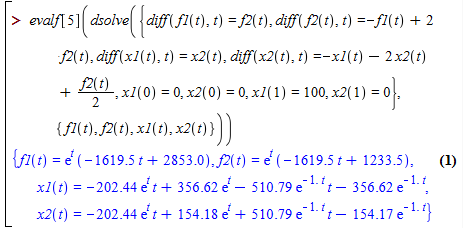
\includegraphics[width=0.6\textwidth]{Maple}
		\caption{Рабочий лист программного пакета \textit{Maple}}
		\label{fig:Maple}
	\end{figure}
	
	Полученная при помощи пакета \textit{MATLAB~Simulink} система представлена на рисунках \ref{fig:system}--\ref{fig:MATLAB-Function}.
	
	\begin{figure}[H]
		\centering
		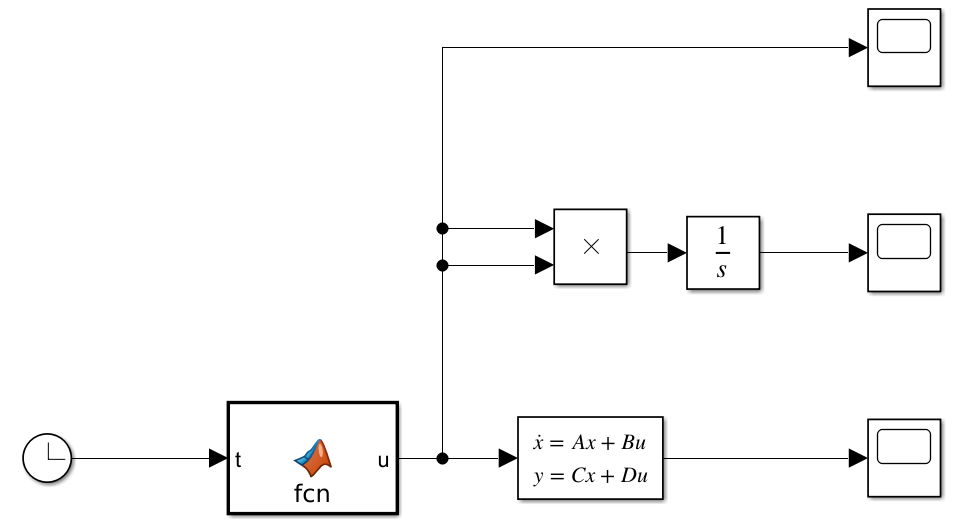
\includegraphics[width=0.6\textwidth]{system}
		\caption{Модель системы}
		\label{fig:system}
	\end{figure}
	
	\begin{figure}[H]
		\centering
		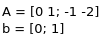
\includegraphics{properties}
		\caption{Параметры системы}
		\label{fig:properties}
	\end{figure}
	
	\begin{figure}[H]
		\centering
		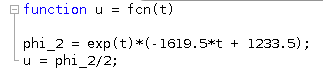
\includegraphics{MATLAB-Function}
		\caption{Блок MATLAB-Function}
		\label{fig:MATLAB-Function}
	\end{figure}
	
	Ниже представлены графики переменных состояния, управления и критерия оптимальности на рисунках \ref{fig:x-2},\ref{fig:u-2} и \ref{fig:J-2} соответственно.
	
	\begin{figure}[H]
		\centering
		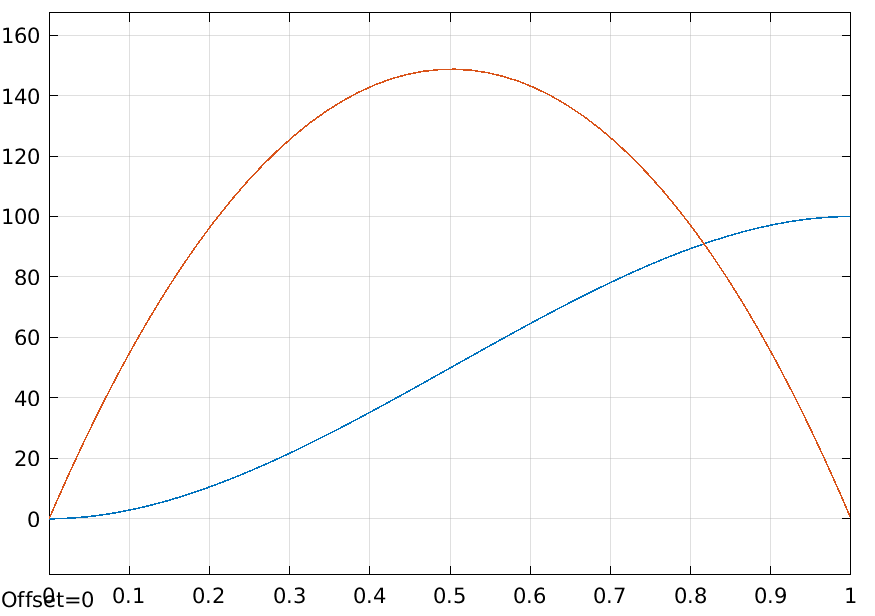
\includegraphics[width=0.6\textwidth]{x-2}
		\caption{Переходный процесс переменных состояния $x$}
		\label{fig:x-2}
	\end{figure}

	\begin{figure}[H]
		\centering
		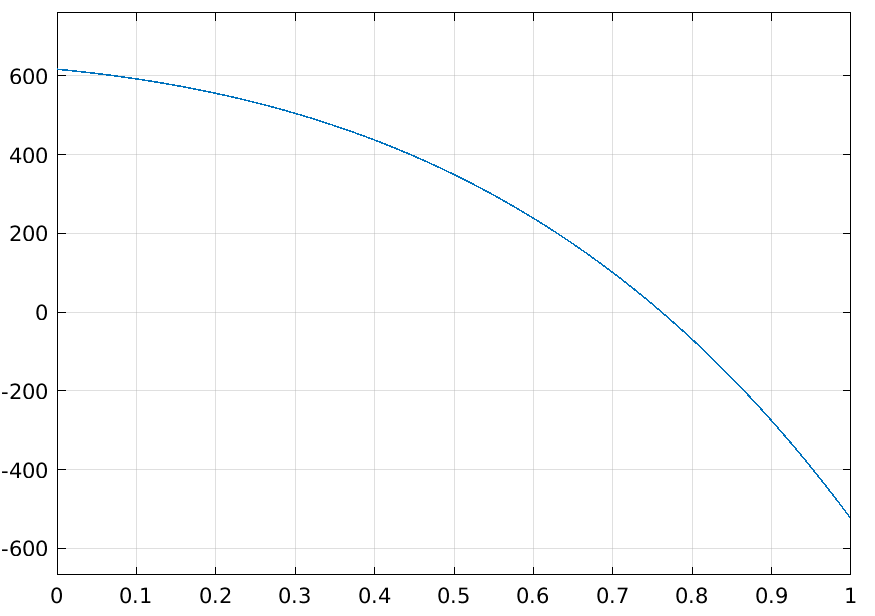
\includegraphics[width=0.6\textwidth]{u-2}
		\caption{Переходный процесс управляющего сигнала $u$}
		\label{fig:u-2}
	\end{figure}

	\begin{figure}[H]
		\centering
		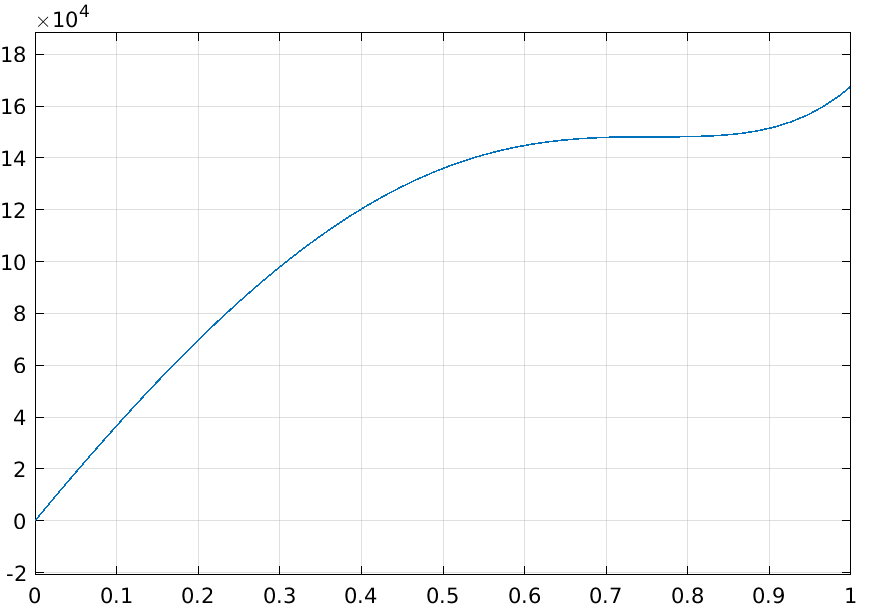
\includegraphics[width=0.6\textwidth]{J-2}
		\caption{Переходный процесс критерия оптимальности $J$}
		\label{fig:J-2}
	\end{figure}	
	
	Теперь произведем моделирование при отклонении параметров регулятора. Отклонять будем управляющий сигнал на 20 значений в положительную и отрицательную стороны. Результаты представлены на рисунках \ref{fig:J-3-plus} и \ref{fig:J-3-minus}.
	
	\begin{figure}[H]
		\centering
		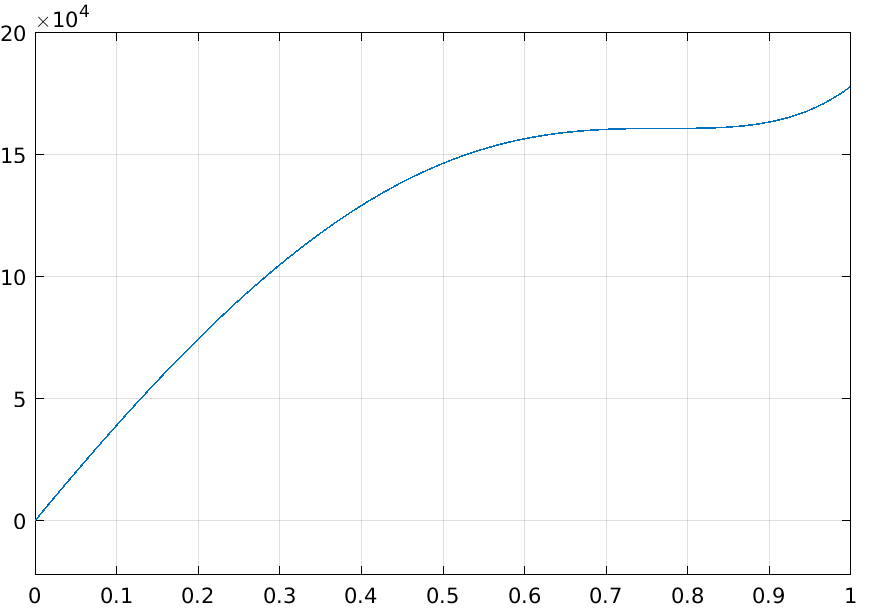
\includegraphics[width=0.6\textwidth]{J-3-plus}
		\caption{Переходный процесс критерия оптимальности $J$ при увеличенном управлении}
		\label{fig:J-3-plus}
	\end{figure}

	\begin{figure}[H]
		\centering
		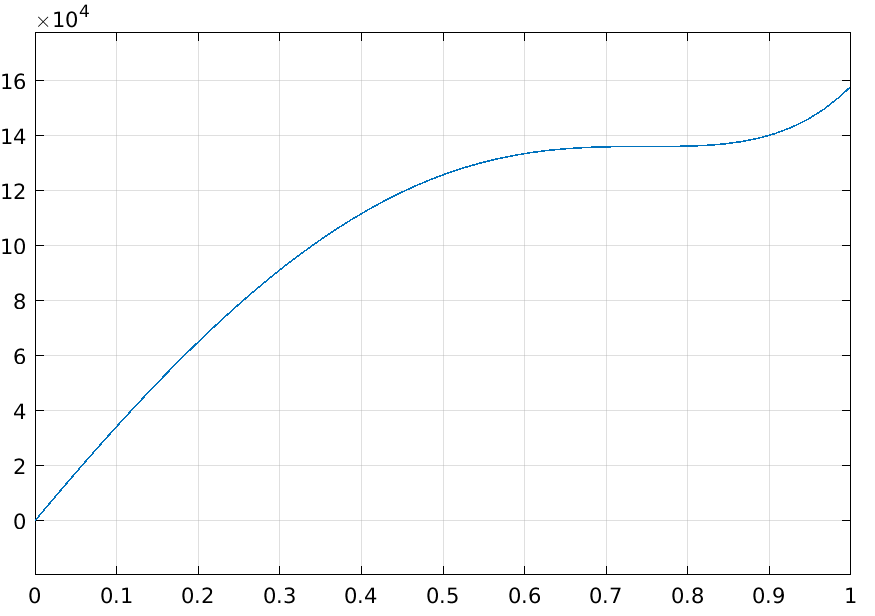
\includegraphics[width=0.6\textwidth]{J-3-minus}
		\caption{Переходный процесс критерия оптимальности $J$ при уменьшенном управлении}
		\label{fig:J-3-minus}
	\end{figure}
	
	\newpage
	
	\section*{Вывод}
	
	Полученный оптимальный в смысле заданного критерия регулятор полностью соответствует заданным условиям.
	
	При отклонении параметров регулятора от оптимальных значений критерий оптимальности изменяется в соответствии с изменением управляющего сигнала. Но при этом конечные значения переменных состояния не достигаются.
	
\end{document}